\documentclass{article}
\usepackage[utf8]{inputenc}
\parskip = 0.75em
\parindent = 10mm
\def\baselinestretch{1}
\usepackage {float}
\usepackage{listings}
\usepackage[usenames]{color}
\usepackage[numbers,sort&compress]{natbib}
\usepackage{multirow, array}
\usepackage[spanish]{babel}
	\deactivatetilden
	\spanishdecimal{.}
	\addto\captionsspanish{\def\tablename{Tabla}}
	\addto\captionsspanish{\def\listtablename{\'Indice de tablas}}

\usepackage{amsmath,amsfonts,amssymb}
	\allowdisplaybreaks[4]
\usepackage{graphicx}
	\graphicspath{{Figuras/}}
\usepackage[clearempty,pagestyles]{titlesec}
\usepackage{anysize}

\def\baselinestretch{1.5}
\papersize{27.9cm}{21.5cm} 
\marginsize{2cm}{2cm}{1cm}{1cm}

\begin{document}


	\begin{center}
	\huge{\textbf{Tarea 1 Simulación del Movimiento Browniano}}
	\line(1,0) {300}\\
	
	\textsc{ \Large Susana Ruiz Nuñez} 
	\textsc{ \Large 2032426}
	\end{center}


\section{Planteamiento del Problema} 
El Movimiento Browniano \cite{satu} se refiere a una partícula cambiando su posición uniformemente al azar. En este trabajo se tratará un caso sencillo donde la partícula se mueve en pasos discretos, es decir, cada paso mide lo mismo, y las únicas posibles direcciones de movimiento son las direcciones paralelas a los ejes cardinales del sistema de coordenadas en el cual se realiza el movimiento.  El objetivo final de este trabajo es examinar de manera sistemática los efectos de la dimensión en el tiempo de regreso al origen del movimiento Browniano para dimensiones 1 a 8 en incrementos lineales de uno, variando el número de pasos de la caminata como potencias de dos con exponente de 5 a 10 (32, 64, 128, 256, 512, 1024) con 50 repeticiones del experimento para cada combinación. Graficar los resultados en una figura con diagramas de caja-bigote, incluir un cuadro indicando el porcentaje de caminatas que nunca regresaron.

\section{Metodología}
Para obtener las caminatas aleatorias necesarias del movimiento browniano se utilizó Python3. Se utilizaron los paquetes de python: random y randint como se muestra en el código a continuación, dicho código es basado en \cite{satu}. Se comprobó primeramente que funcionara para una dimensión y luego se fue observando el comportamiento hasta 8 dimensiones, variando a su vez el número de pasos de la caminata comenzando en potencia de dos con exponente 5 y terminando en potencia de dos con exponente 10. Como el objetivo era conocer el número de pasos que daba la caminata para regresar al origen, se detiene la misma cuando llega a su posición inicial(el origen) y se imprime el número de pasos.
  
\begin{lstlisting}[language=Python]
	def caminata(currentPos, dimentions):
		nextPos = currentPos[:]
		randomDimention = randint(0, dimentions-1)
		nextPos[randomDimention] += -1 if random() < 0.5 else 1
		return nextPos
	
	initialPos = [0] * dimentions
	currentPos = initialPos
	
	for stepNumber in range(steps):
		currentPos = caminata(currentPos, dimentions)
		if (currentPos == initialPos):
			break
	print(stepNumber)
\end{lstlisting}

     
\section{Resultados obtenidos}
Repetidas las pruebas para todas las dimensiones y para todos los pasos de la caminata, se obtuvieron valores del porcentaje de la cantidad de veces que retornaba al origen la partícula. El comportamiento de la partícula para todas las pruebas hechas se observa en un diagrama de caja-bigote(Figura 1), cuyo eje horizontal está representado por las dimensiones (1-8) y el eje vertical por el porcentaje obtenido de regreso de la partícula al origen. Como se observa en el comportamiento, se hace más difícil a la partícula regresar al  aumentar las dimensiones, teniendo que para la dimensión 1, la probabilidad de regreso es muy alta, casi alcanza el 100 por ciento, mientras que para la última dimensión estudiada, la partícula no retorna casi nunca.

\begin{figure}[H]
    \centering

    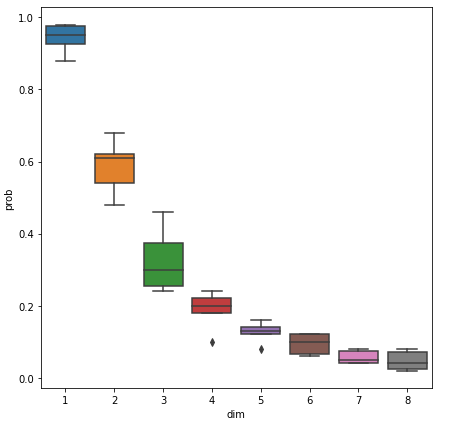
\includegraphics[scale=0.6]{Caja.png}
    \caption{Diagrama de caja-bigote para 8 dimensiones}
    \label{fig:f1}
\end{figure}

Este mismo análisis se desarrolló para el conteo de números de pasos que le demoraba a la partícula retornar al origen (Figura 2). Explorando de igual manera las 8 dimensiones y cambiando el número de pasos desde 32 hasta 1024. Se observa tanto en la figura 1 como en la 2, que existen valores picos, que quedan fuera de la caja; esto ocurre porque se nota una dispersión en los valores de retorno, lo mismo se retornaba en un paso que en 128. Este comportamiento se nota sobre todo para las pruebas pequeñas, para las pruebas de instancias más grandes se mantiene un comportamiento más uniforme.

\begin{figure}[H]
	\centering
	
	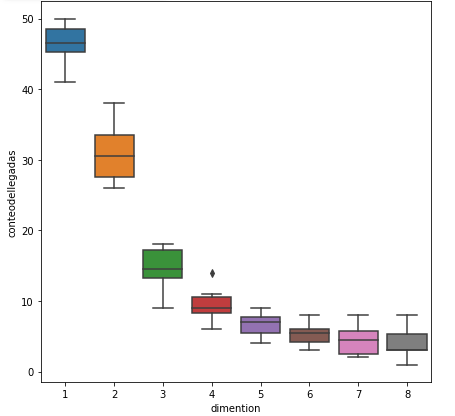
\includegraphics[scale=0.6]{Pasosdellegada.png}
	\caption{Pasos para llegar al origen}
	\label{fig:f2}
\end{figure}

A continuación se muestra también de los datos recopilados, un cuadro indicando el porciento de las caminatas que nunca regresaron al origen para todas las dimensiones. Se fortalece lo mencionado con anterioridad, que para una dimensión y para dimensiones pequeñas le es más fácil retornar al origen, por eso tienen porcientos tan bajos de no retorno.
\begin{center}
\begin{tabular}{|c|c|c|c|}
\hline 
Dimensión & Porcentaje de no retorno \\ 
\hline 
1 & 0.06 \\ 
\hline 
2 & 0.4 \\ 
\hline 
3 & 0.7 \\ 
\hline 
4 & 0.82 \\ 
\hline 
5 & 0.8 \\ 
\hline 
6 & 0.91 \\ 
\hline 
7 & 0.94 \\ 
\hline 
8 & 0.96 \\ 
\hline
\end{tabular}
\end{center}
\begin{center}
	Tabla 1: Porcentaje de las caminatas que no regresan al origen
\end{center}

Además de observar el comportamiento colectivo de las dimensiones y sus variaciones en los diferentes tamaños de las caminatas. Se hizo un análisis individual para cada dimensión. Se muestran en las figuras posteriores el número de pasos de vuelta al origen para la caminata más pequeña (Figura 3) y para la de mayor número de pasos (Figura 4).

\begin{figure}[H]
	\centering
	
	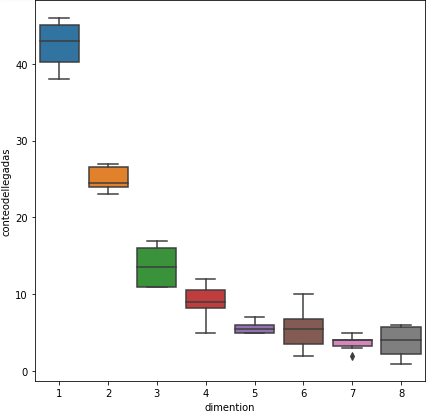
\includegraphics[scale=0.5]{Llegadapasos32.png}
	\caption{Pasos para llegar al origen de la caminata de 32 pasos}
	\label{fig:f3}
\end{figure}

\begin{figure}[H]
	\centering
	
	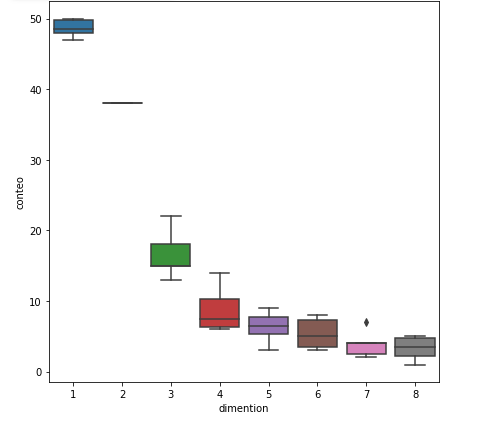
\includegraphics[scale=0.5]{Llegadadepasos1024.png}
	\caption{Pasos para llegar al origen de la caminata de 1024 pasos}
	\label{fig:f4}
\end{figure}
 
\section{Conclusiones}
Se puede concluir con los experimentos realizados que se hace más complejo el regreso de la partícula mientras aumentan las dimensiones, por el contrario se hace más estable el experimento al aumentar los pasos. Este análisis fue realizado para la caminata Manhattan, es necesario continuar trabajando y realizar pruebas para la Euclediana, además de hacer un mayor número de pruebas para lograr ver el comportamiento en fracciones de tiempo pequeñas. 

\bibliography{Tarea1}
\bibliographystyle{plainnat}
\end{document} 
